
\section{Exploring the latent space of StyleGAN}
\label{stylegan}

In this section we will explore  very recent advances in face synthesis and semantic face editing\footnote{The InterfaceGan paper was published July this year!} by using a pretrained StyleGan trained by Nvidia. 

We can download the weigths of a pretrained stylegan trained by Nvidia directly from their Github. \footnote{\url{https://github.com/NVlabs/stylegan.git}}\cite{stylegan}
This model is trained on the full size and resolution version of the FFHQ dataset.
With the trained generator we can draw sample $z$ from the normal distribution and generate faces $G(x)$ which are near impossible to humans to distinguish from real faces.

In Figure \ref{StyleGAN-examples} we see eight such samples. We can create as many photo realistic faces, of people who have existed, as we want.
\begin{figure}[h!]
  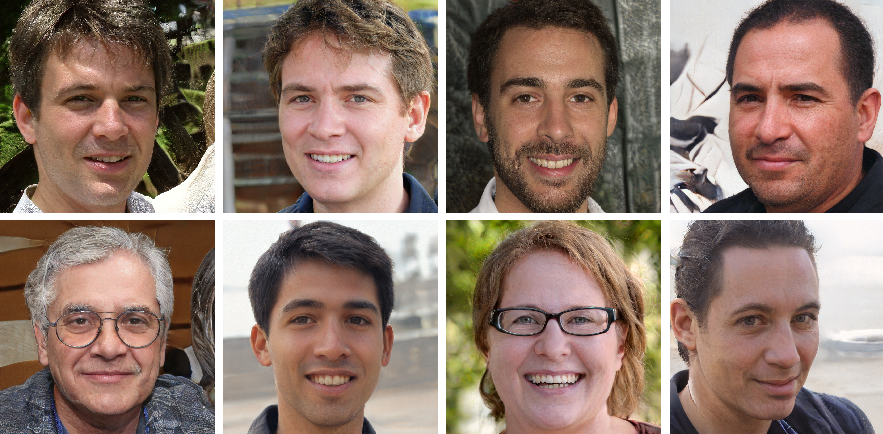
\includegraphics[width=\textwidth]{fig/stylegan/randomsamples}
  \caption{Random samples from the pretrained StyleGAN}
  \label{StyleGAN-examples}
\end{figure}




\subsection{Finding the latent space representation of an arbitrary query image.}
Now the pretrained StyleGAN does not contain an encoder network. Therefore there is no way to find a latent space representation of a arbitrary input image.
There is, however a a least two different ways of tackling this problem.
%
% One is the optimization-based
% approach, which directly optimizes the latent code with fixed generator to minimize the pixel-wise reconstruction error [22]. The other is the encoder-based, where an independent encoder network is trained to learn the inverse mapping [37].
\cite{interfacegan}
The paper \textit{Image2StyleGAN: How to Embed Images Into the StyleGAN Latent Space?}\cite{Image2StyleGAN} explicitly investigates this problem.


Here we use the first approach where hold the pretrained generator fixed and then optimize the latent vector to give the desired output image. But instead of calculating the loss directly on the pixel-wise reconstruction error. \footnote{Here we use the codebase provided at: \url{https://github.com/Puzer/stylegan-encoder}}

Here we use the same approach as in \cite{styletransfer} where

We use a pre-trained VGG16 network for transforming a query image and the generated image from the latent vector into a high dimensional feature space. The loss is them calculated as a difference between the two feature vectors in the VGG16 feature space.

\begin{figure}
    \centering
    \begin{subfigure}[b]{\textwidth}
        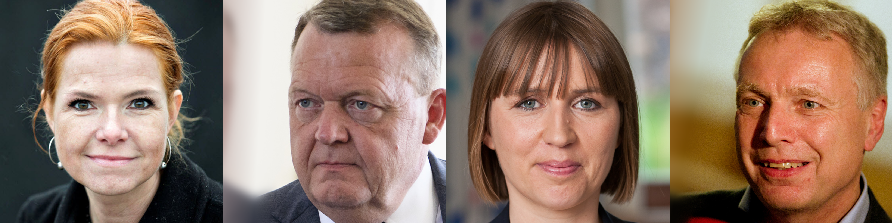
\includegraphics[width=\textwidth]{fig/stylegan/originals}
        \caption{Original images.}
    \end{subfigure}
        \begin{subfigure}[b]{\textwidth}
        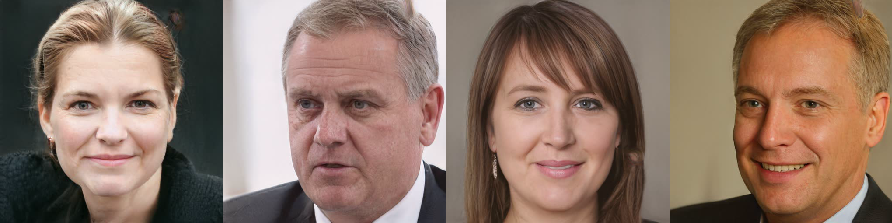
\includegraphics[width=\textwidth]{fig/stylegan/reconstructionsfirstguess.png}
        \caption{First guess of the latent space representation using the pretrained ResNet network}
    \end{subfigure}
    \begin{subfigure}[b]{\textwidth}
        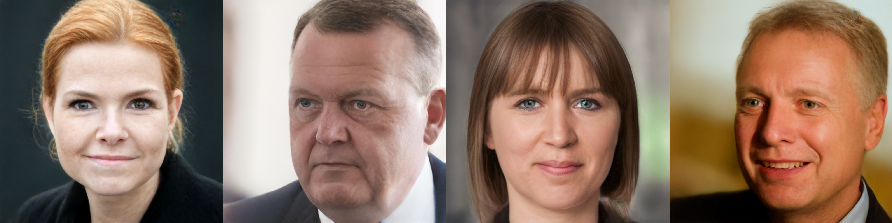
\includegraphics[width=\textwidth]{fig/stylegan/reconstructions}
        \caption{The reconstructed images after optimization using the pretrained VGG16 network.}
    \end{subfigure}
    \caption{Comparison of original query images and their reconstruction in the StyleGAN network}
    \label{stylegan-reconstruction}
\end{figure}

We can to a linear interpolation between two latent vectors $z_1$ and $z_2$ simply by
\begin{align}
  z = \alpha z_2 + (1-\alpha)z_1
\end{align}
for $0 \leq \alpha \leq 1$. This linear interpolation results in images that smoothly transitions between faces generated by $z_1$ and $z_2$ respectively. In Figure \ref{StyleGAN-interpolation} we see the result of doing a linear interpolation between the latent representations of the two last danish prime ministers.

\begin{figure}
  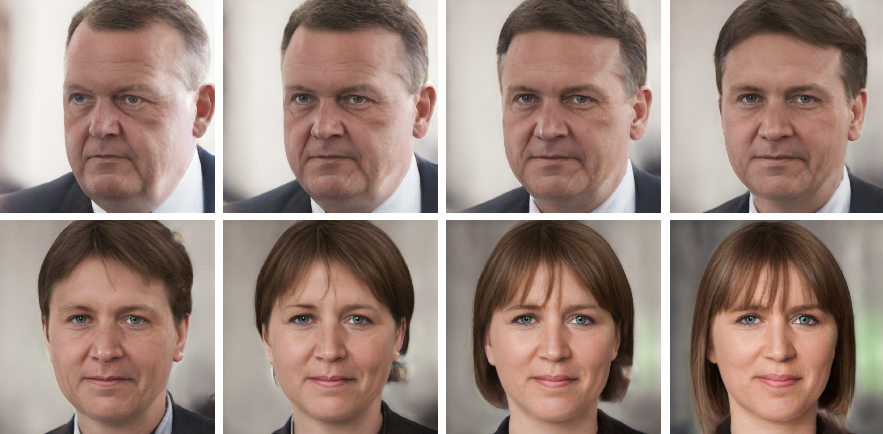
\includegraphics[width=\textwidth]{fig/stylegan/interpolation}
  \caption{Interpolation between two StyleGAN images}
  \label{StyleGAN-interpolation}
\end{figure}


% Optimization is performed only for latent representation which we want to obtain.

% Upon completion of optimization you are able to transform your latent vector as you wish. For example you can find a "smiling direction" in your latent space, move your latent vector in this direction and transform it back to image using the generator.

%
% \begin{figure}[htb]
%     \centering
%     \begin{subfigure}[b]{\textwidth}
%         \centering
%         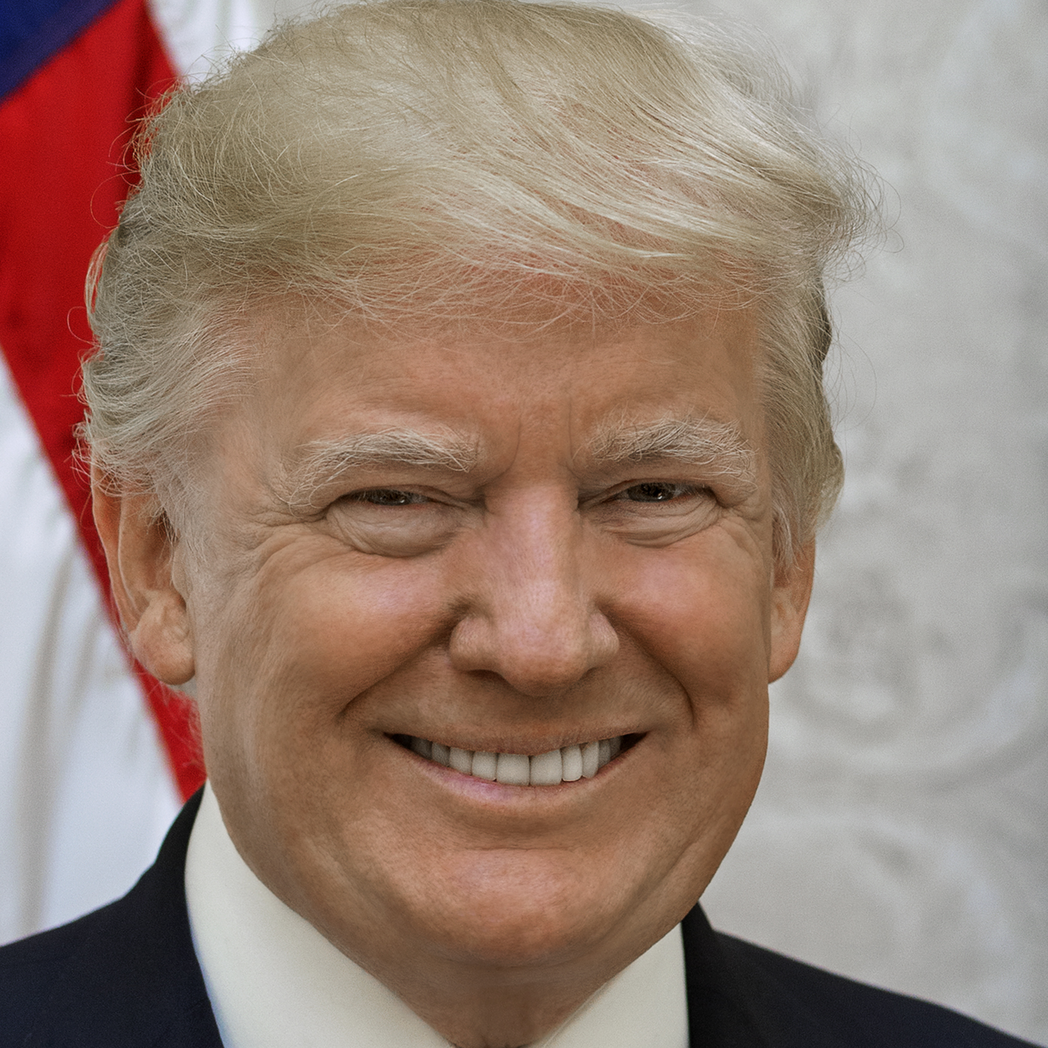
\includegraphics[width=0.3\linewidth]{fig/query_images/trump}%
%         \hfill
%         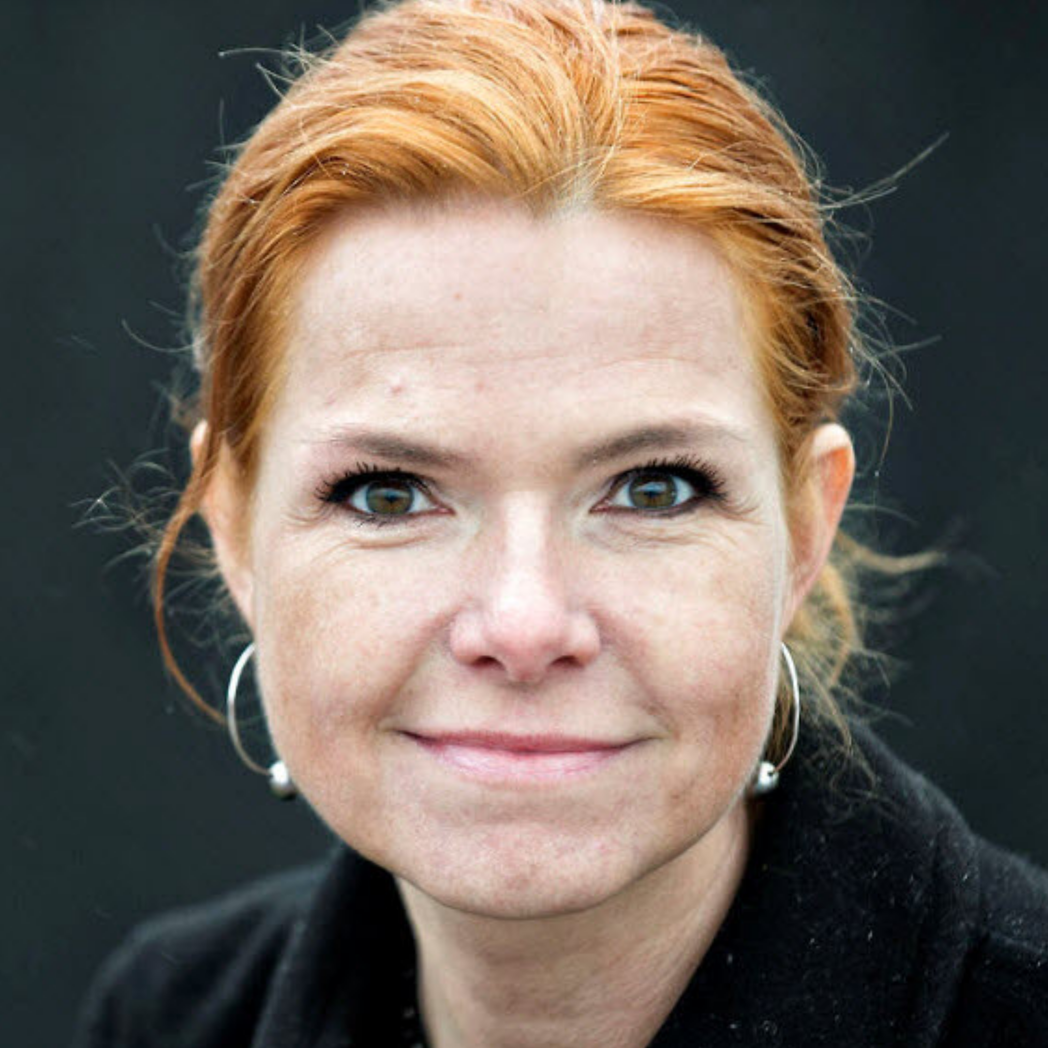
\includegraphics[width=0.3\linewidth]{fig/query_images/inger}
%         \hfill
%         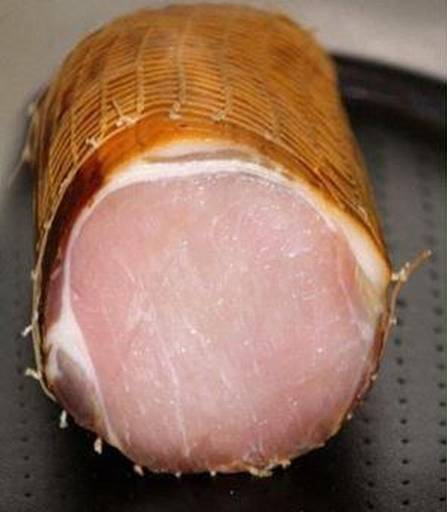
\includegraphics[width=0.3\linewidth]{fig/query_images/skinke}
%         \caption{Original Query Images}
%     \end{subfigure}
%     \vskip\baselineskip
%     \begin{subfigure}[b]{\textwidth}
%         \centering
%         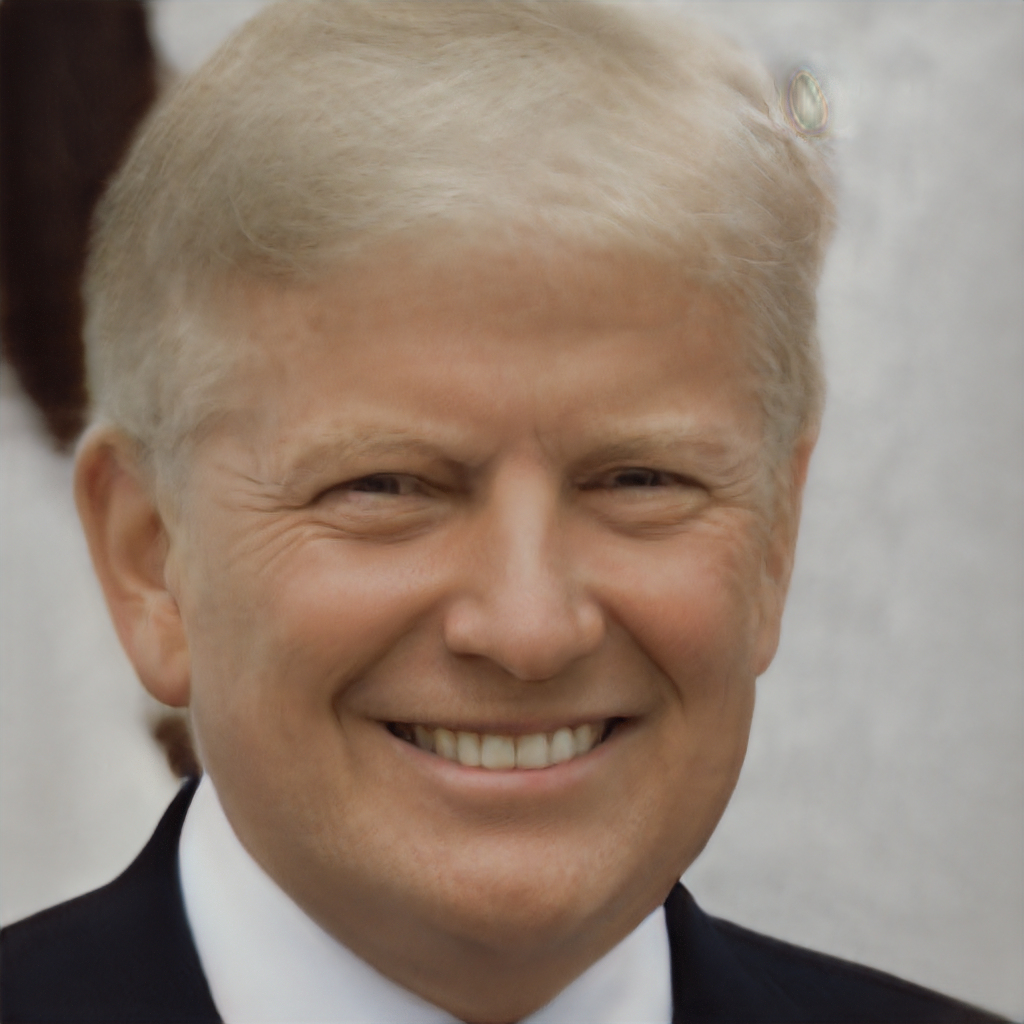
\includegraphics[width=0.3\linewidth]{fig/query_images_reconstucted/trump}%
%         \hfill
%         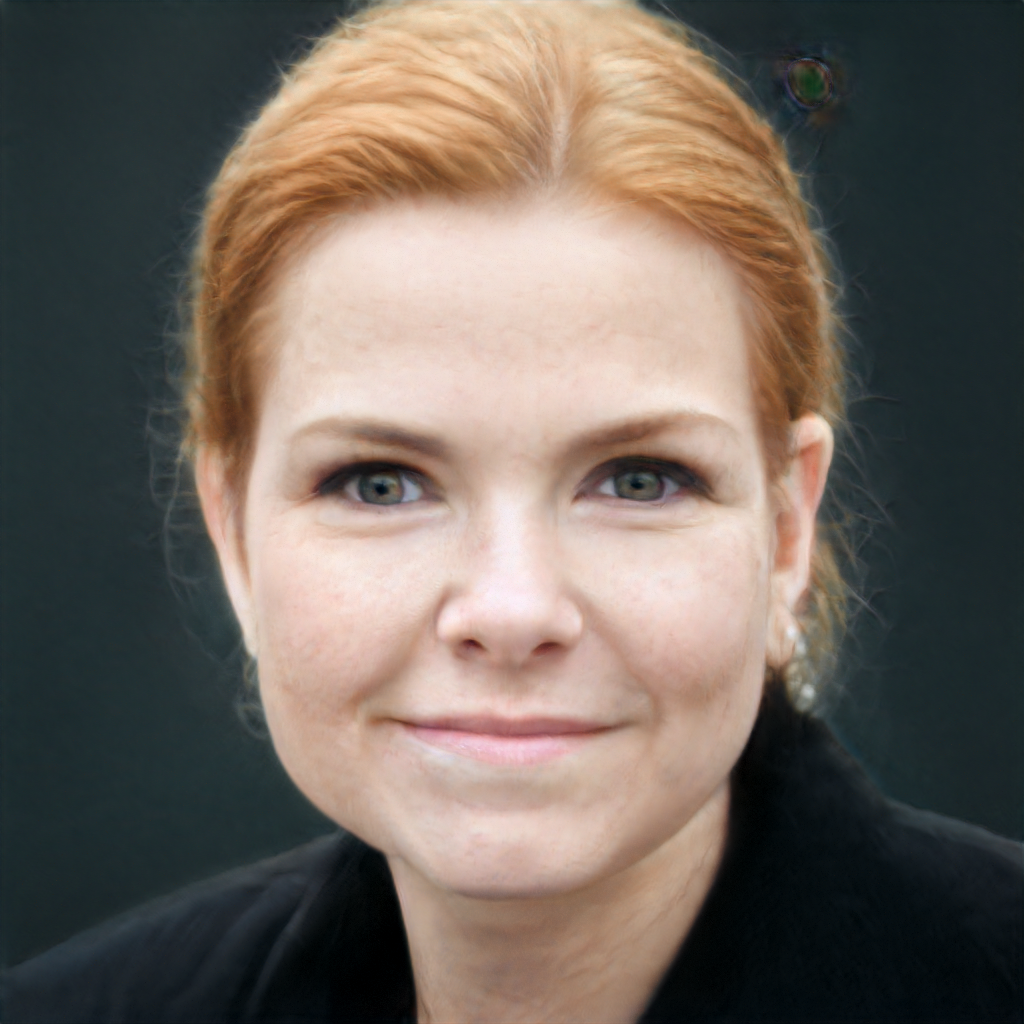
\includegraphics[width=0.3\linewidth]{fig/query_images_reconstucted/inger}
%         \hfill
%         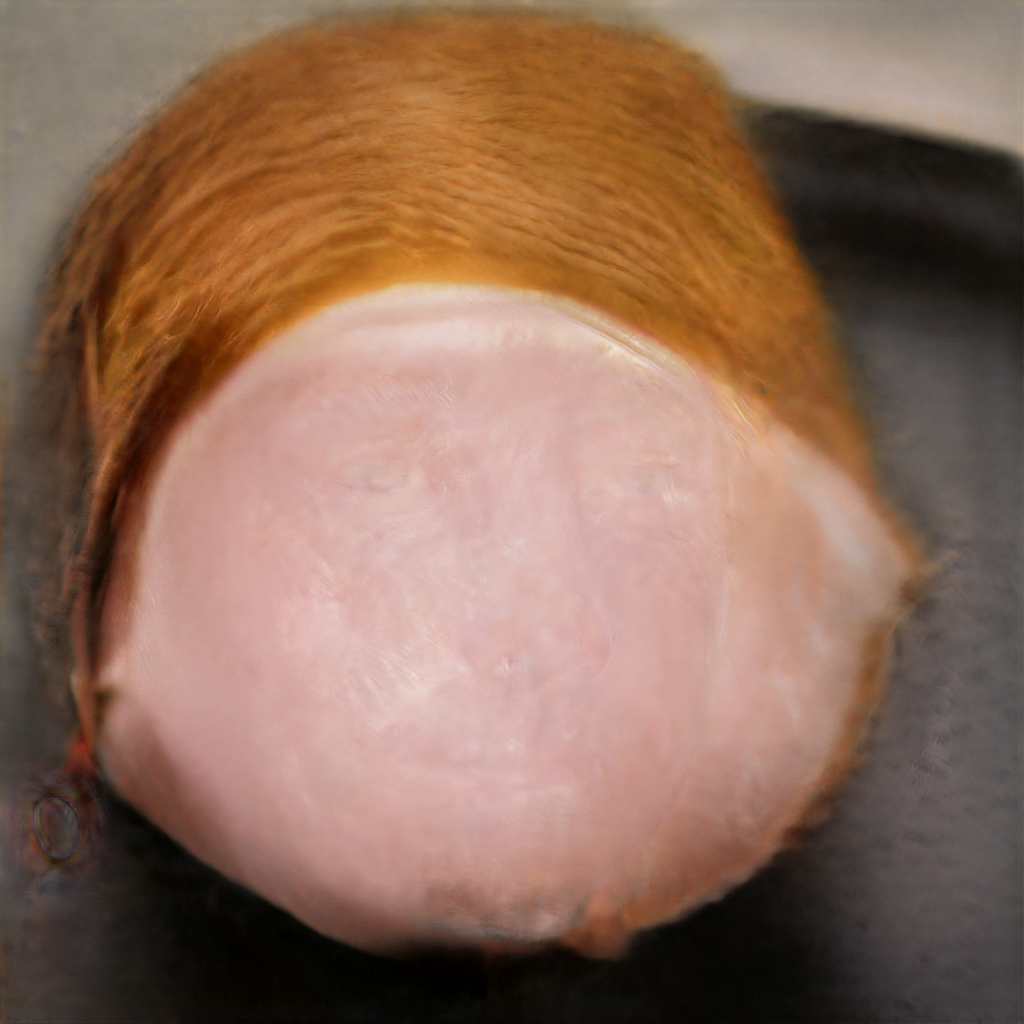
\includegraphics[width=0.3\linewidth]{fig/query_images_reconstucted/skinke}
%         \caption{Reconstructed images from StyleGAN latent space}
%     \end{subfigure}
%     \caption{Latent space representation of arbitrary query images }
% \end{figure}

% \begin{figure}
%     \centering
%     \begin{subfigure}[b]{0.45\textwidth}
%         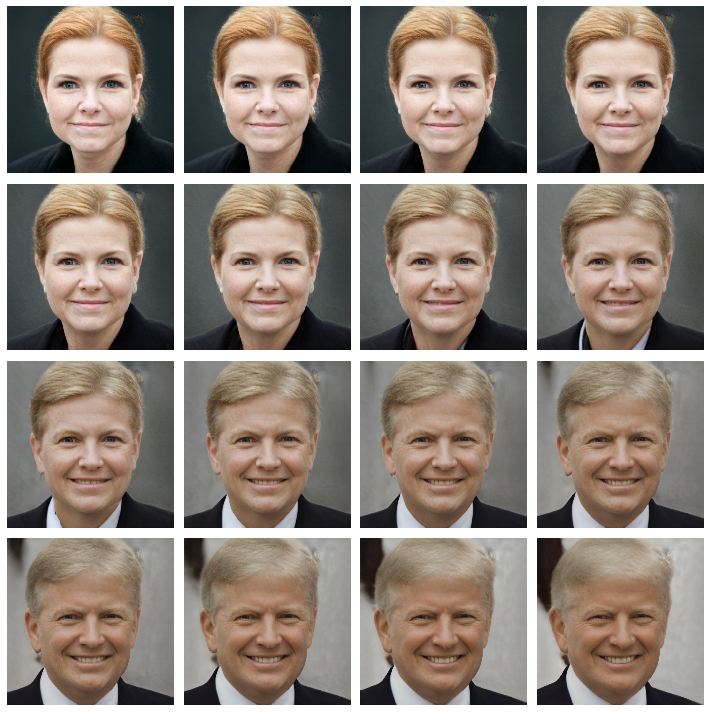
\includegraphics[width=\textwidth]{fig/ingertrump}
%         \caption{Inger Støjberg to Donald Trump}
%     \end{subfigure}
%     ~
%     \begin{subfigure}[b]{0.45\textwidth}
%         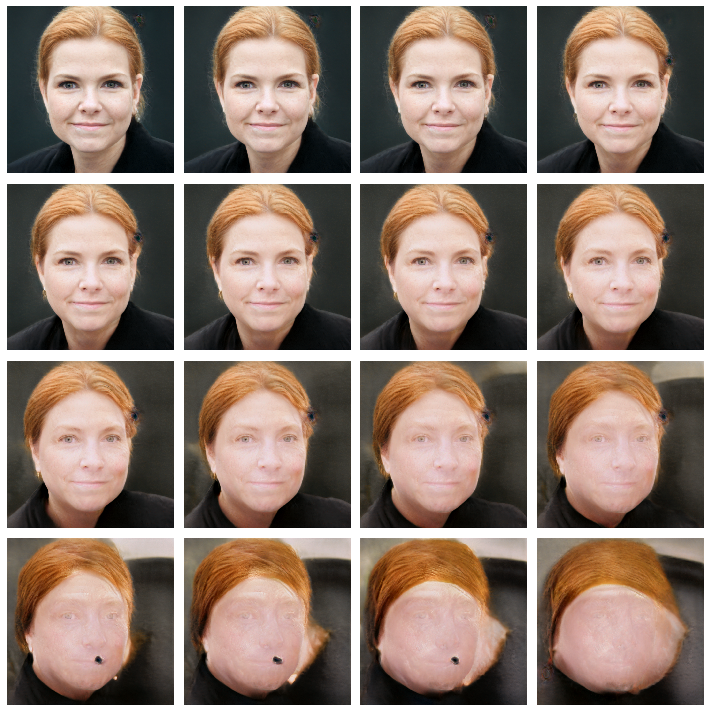
\includegraphics[width=\textwidth]{fig/ingerham}
%         \caption{Inger Støjberg to Ham}
%     \end{subfigure}
%     \caption{Interpolations between query images in the StyleGAN latent space.}
% \end{figure}

\subsection{Semantic face editing.}

In Figure \ref{faceedit} we see the results from doing semantic face editing of the reconstructed images from
\ref{stylegan-reconstruction}.

\begin{figure}[h!]
    \centering
    \begin{subfigure}[b]{0.24\textwidth}
        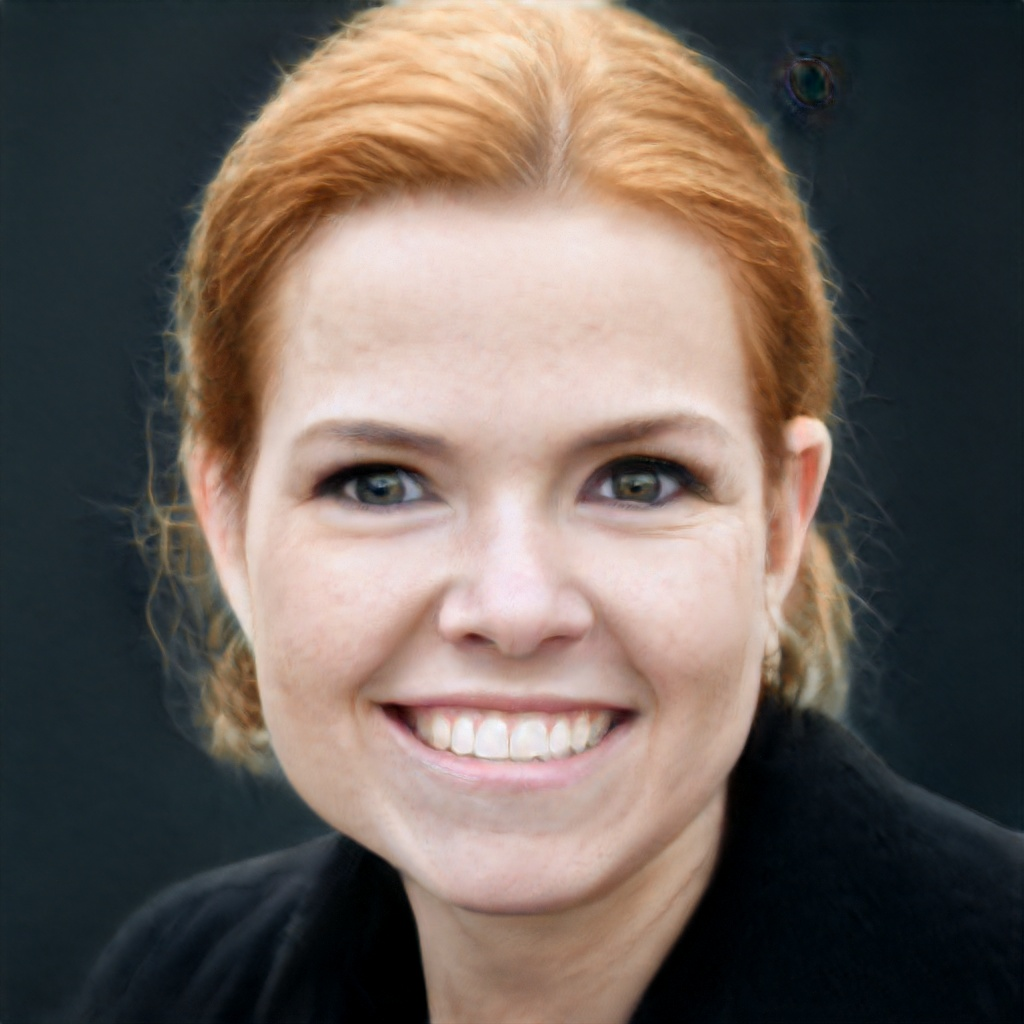
\includegraphics[width=\textwidth]{fig/stylegan/faceedit/inger-smile}
    \end{subfigure}
    \begin{subfigure}[b]{0.24\textwidth}
        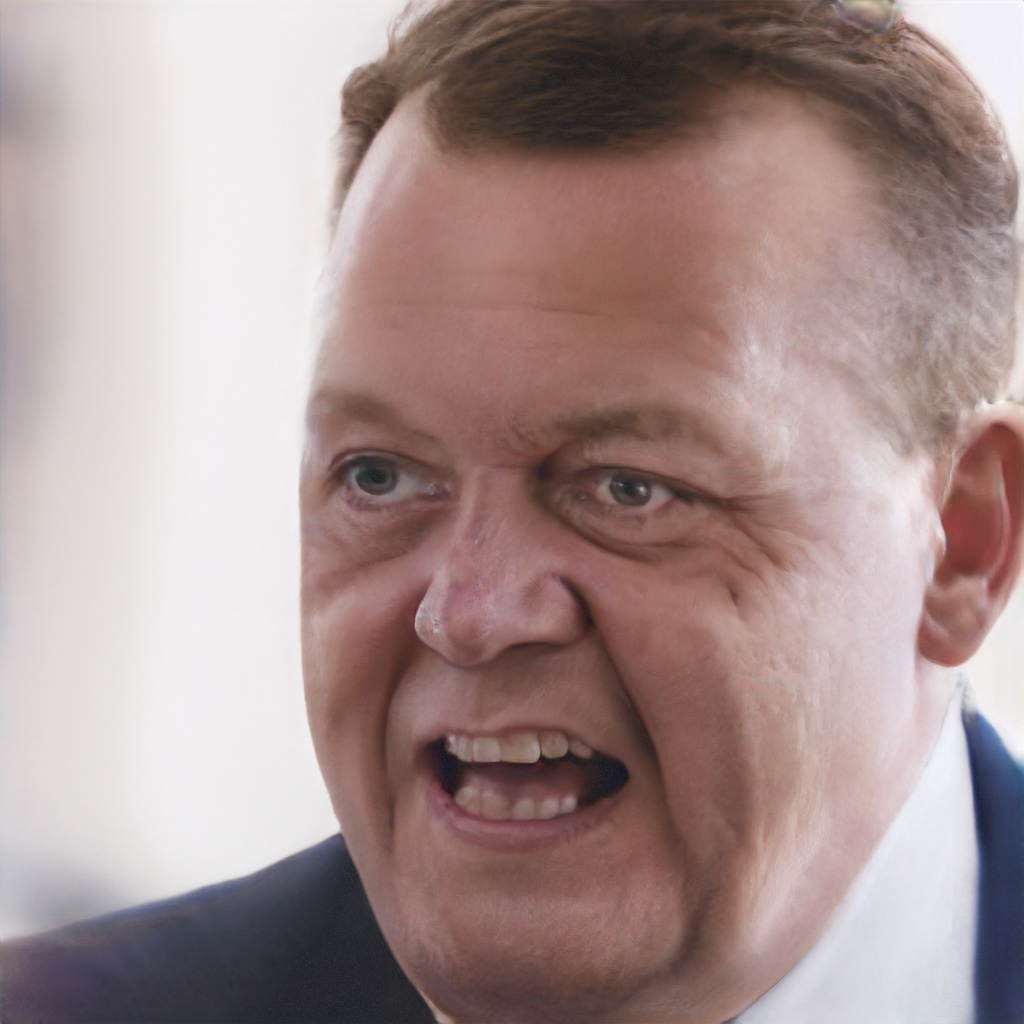
\includegraphics[width=\textwidth]{fig/stylegan/faceedit/lars-smile}
    \end{subfigure}
    \begin{subfigure}[b]{0.24\textwidth}
        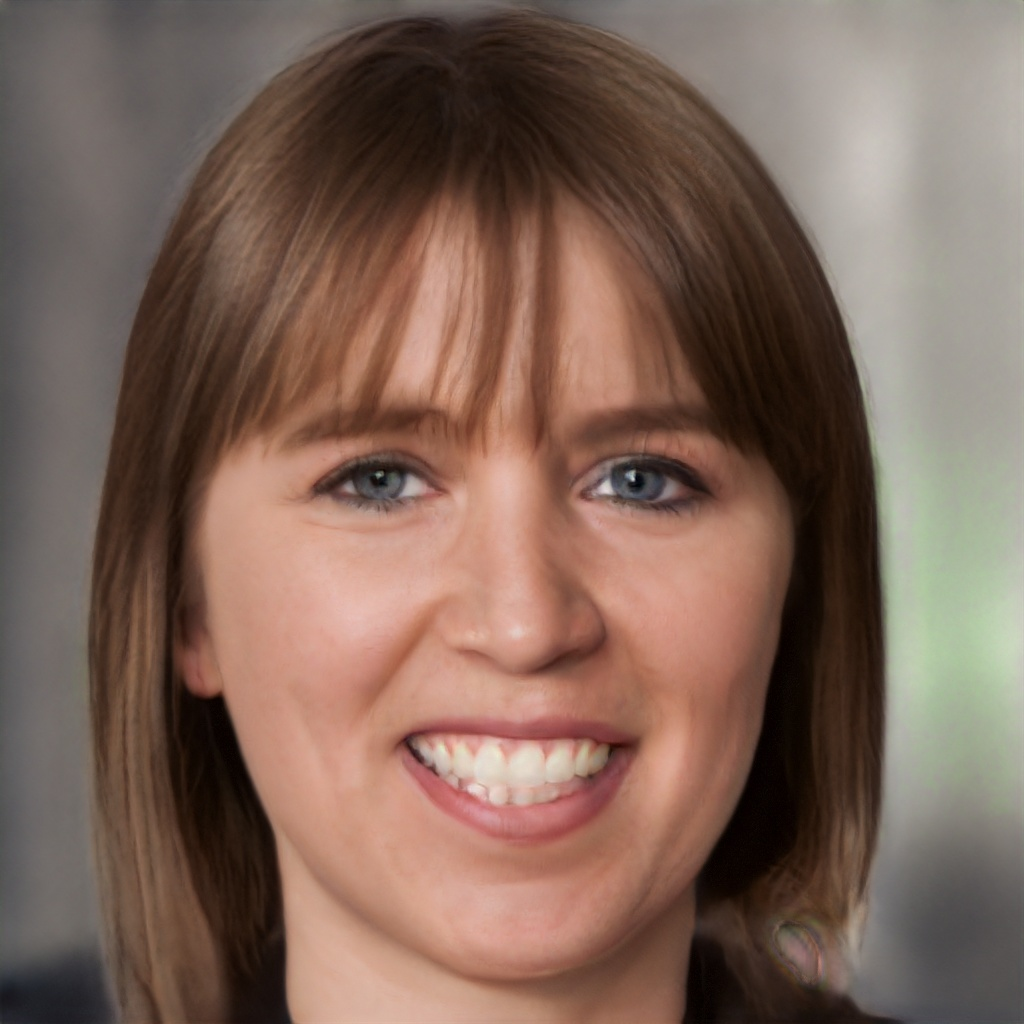
\includegraphics[width=\textwidth]{fig/stylegan/faceedit/mette-smile}
    \end{subfigure}
    \begin{subfigure}[b]{0.24\textwidth}
        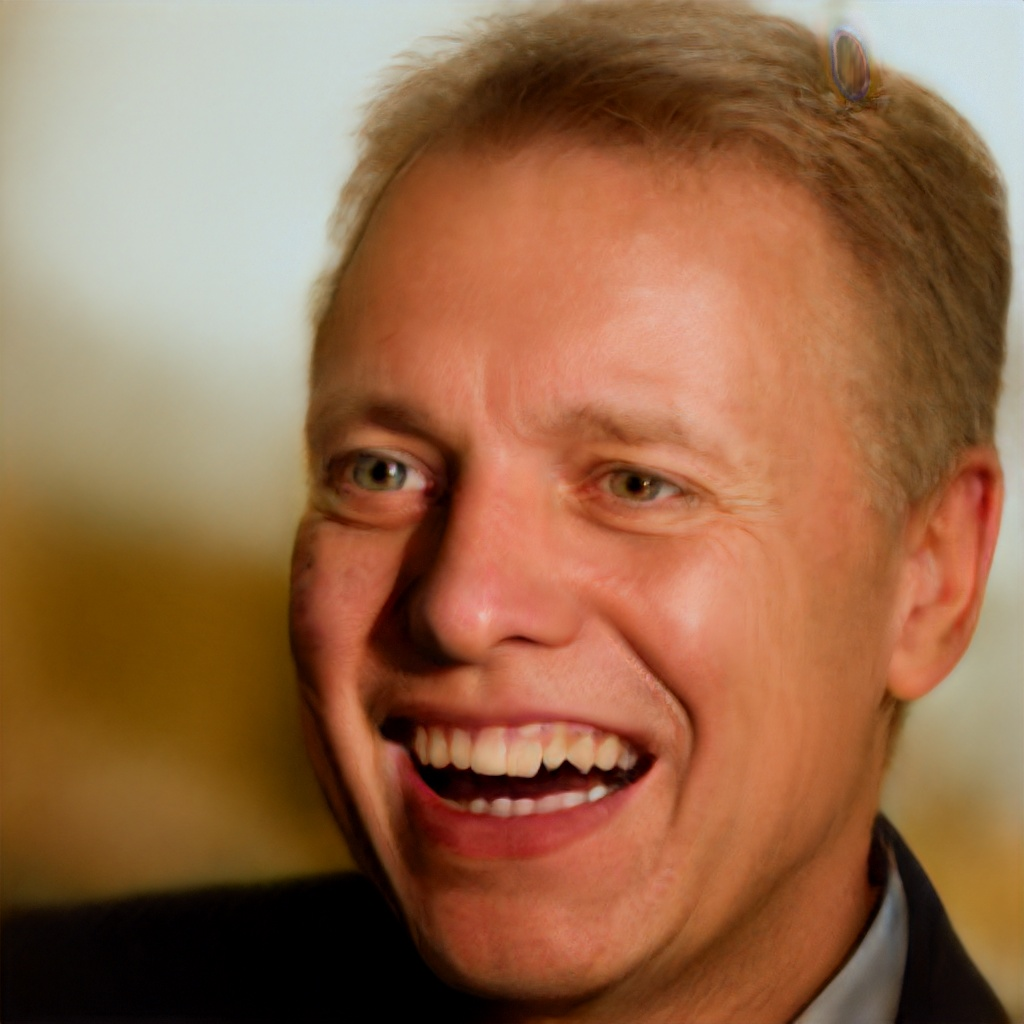
\includegraphics[width=\textwidth]{fig/stylegan/faceedit/uffe-smile}
    \end{subfigure}
    \begin{subfigure}[b]{0.24\textwidth}
        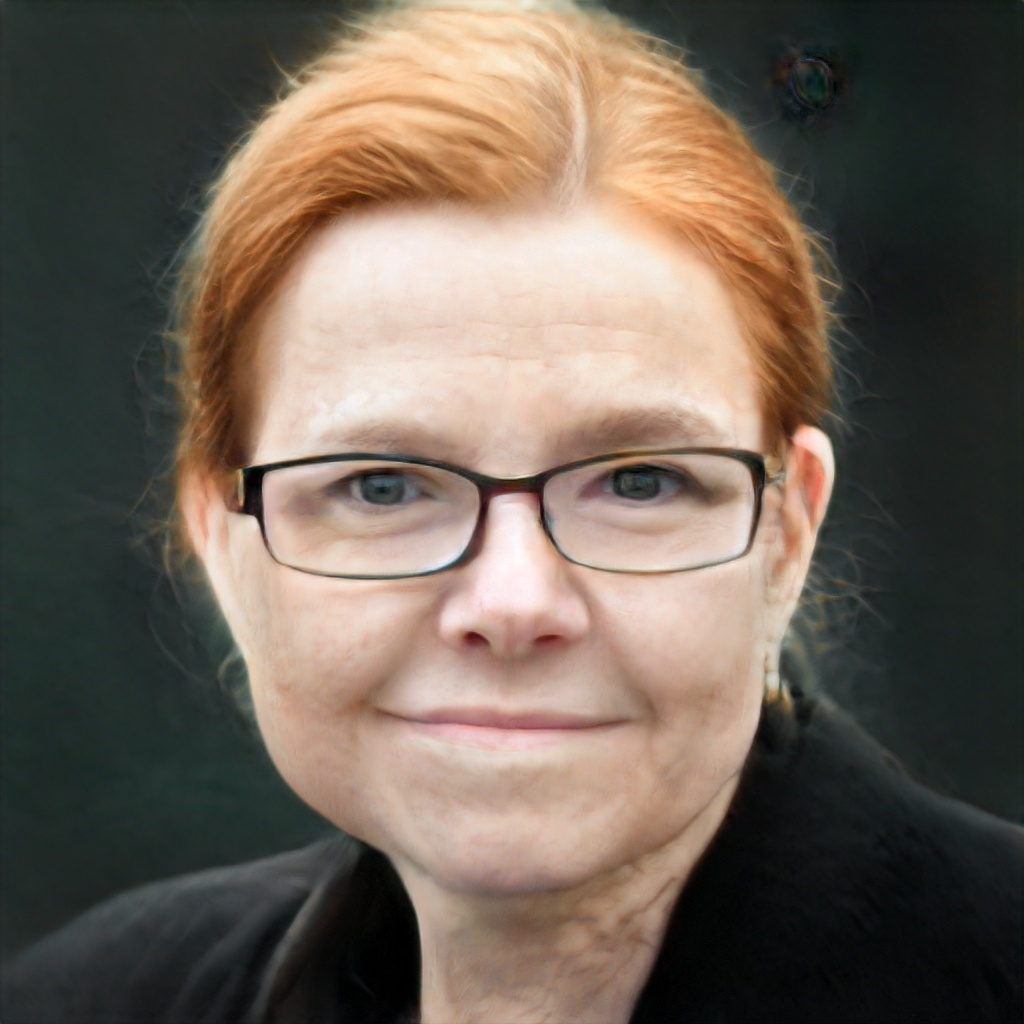
\includegraphics[width=\textwidth]{fig/stylegan/faceedit/inger-glasses}
    \end{subfigure}
    \begin{subfigure}[b]{0.24\textwidth}
        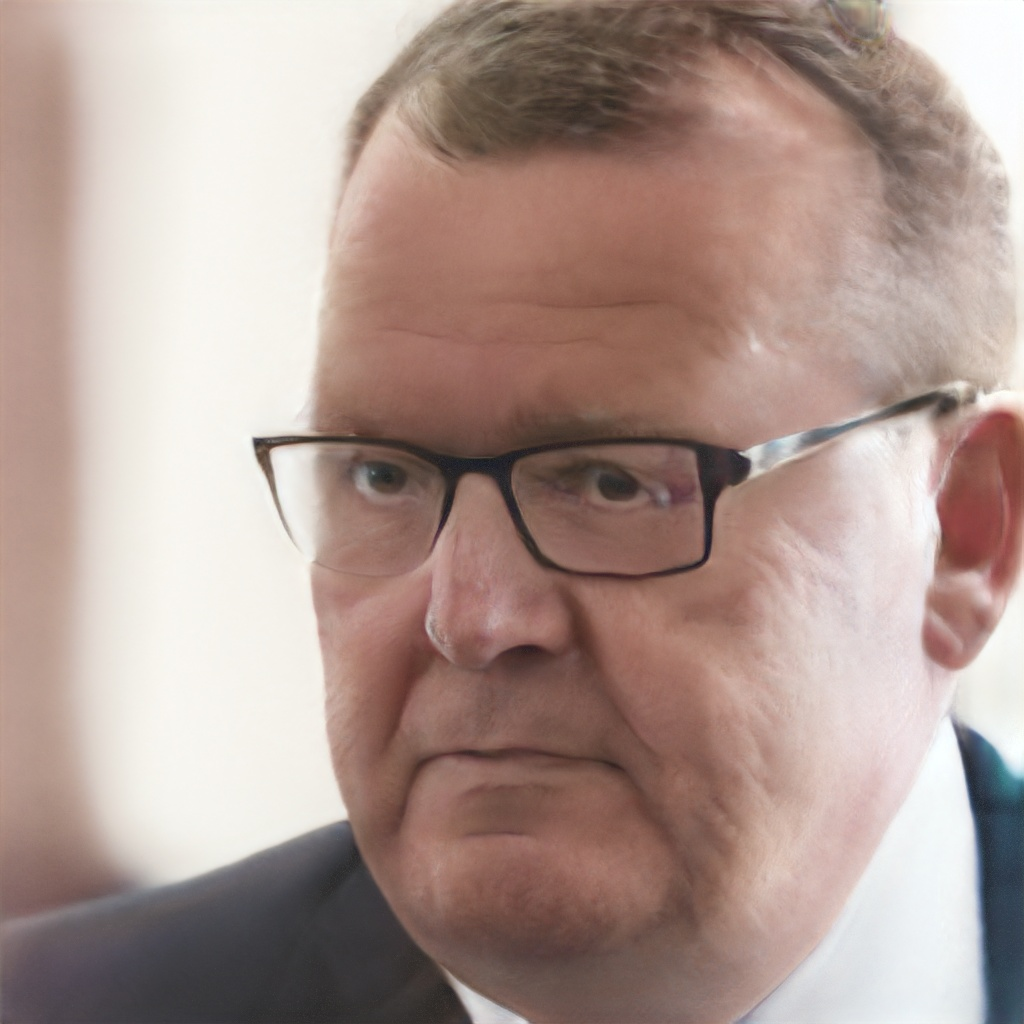
\includegraphics[width=\textwidth]{fig/stylegan/faceedit/lars-glasses}
    \end{subfigure}
    \begin{subfigure}[b]{0.24\textwidth}
        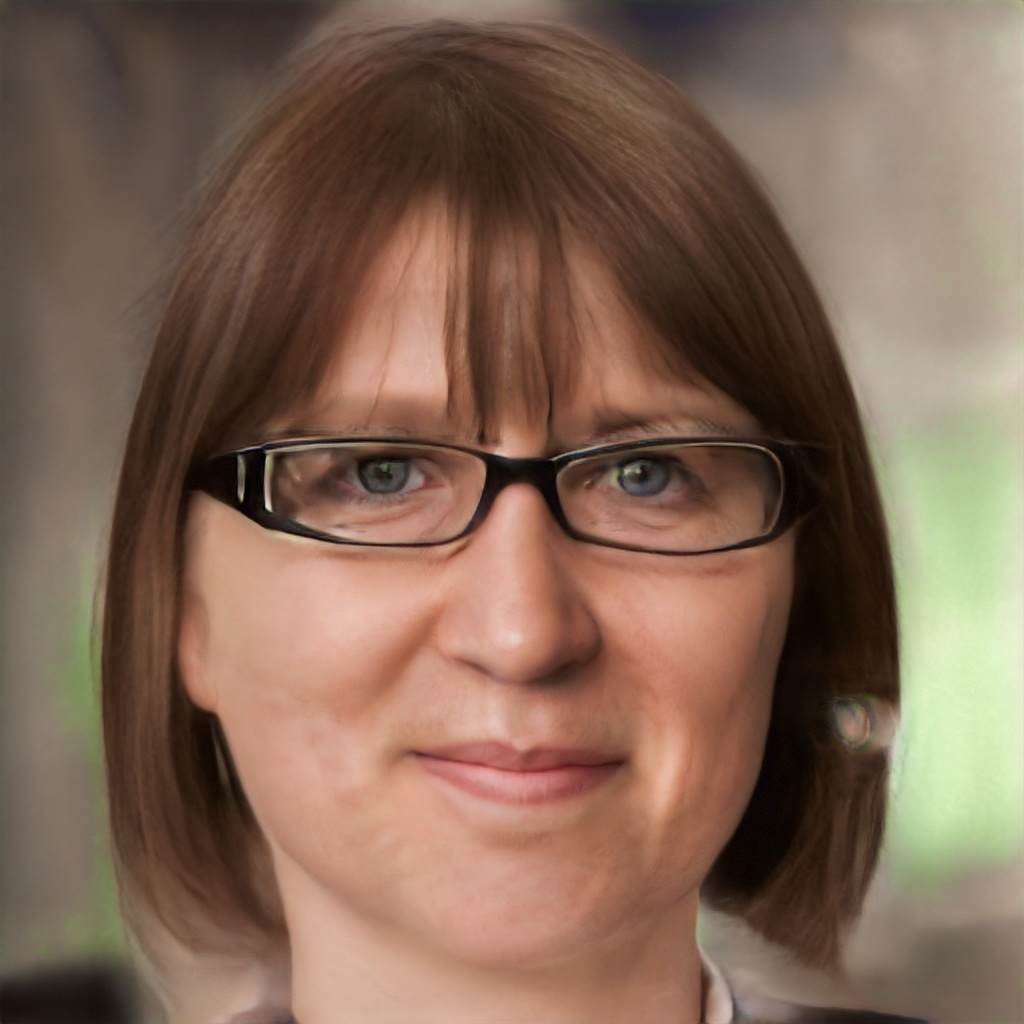
\includegraphics[width=\textwidth]{fig/stylegan/faceedit/mette-glasses}
    \end{subfigure}
    \begin{subfigure}[b]{0.24\textwidth}
        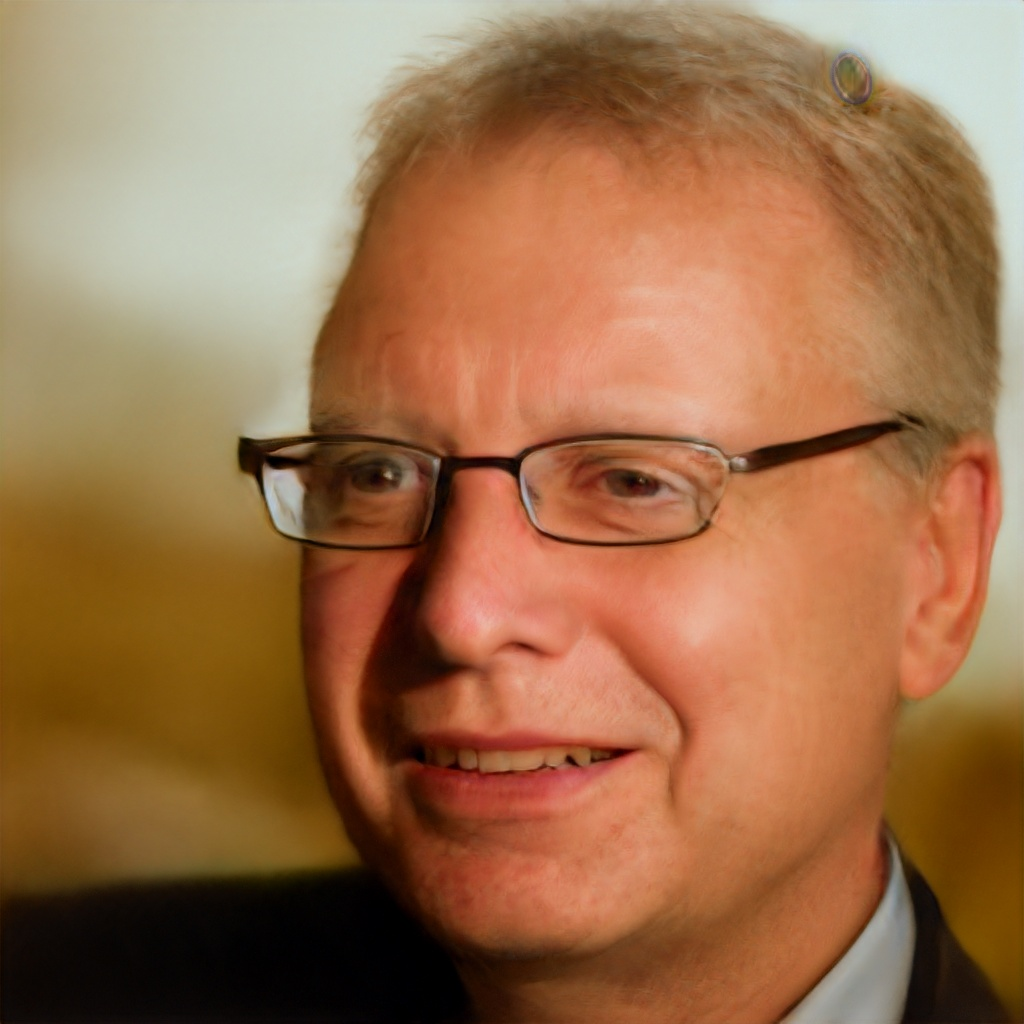
\includegraphics[width=\textwidth]{fig/stylegan/faceedit/uffe-glasses}
    \end{subfigure}
    \begin{subfigure}[b]{0.24\textwidth}
        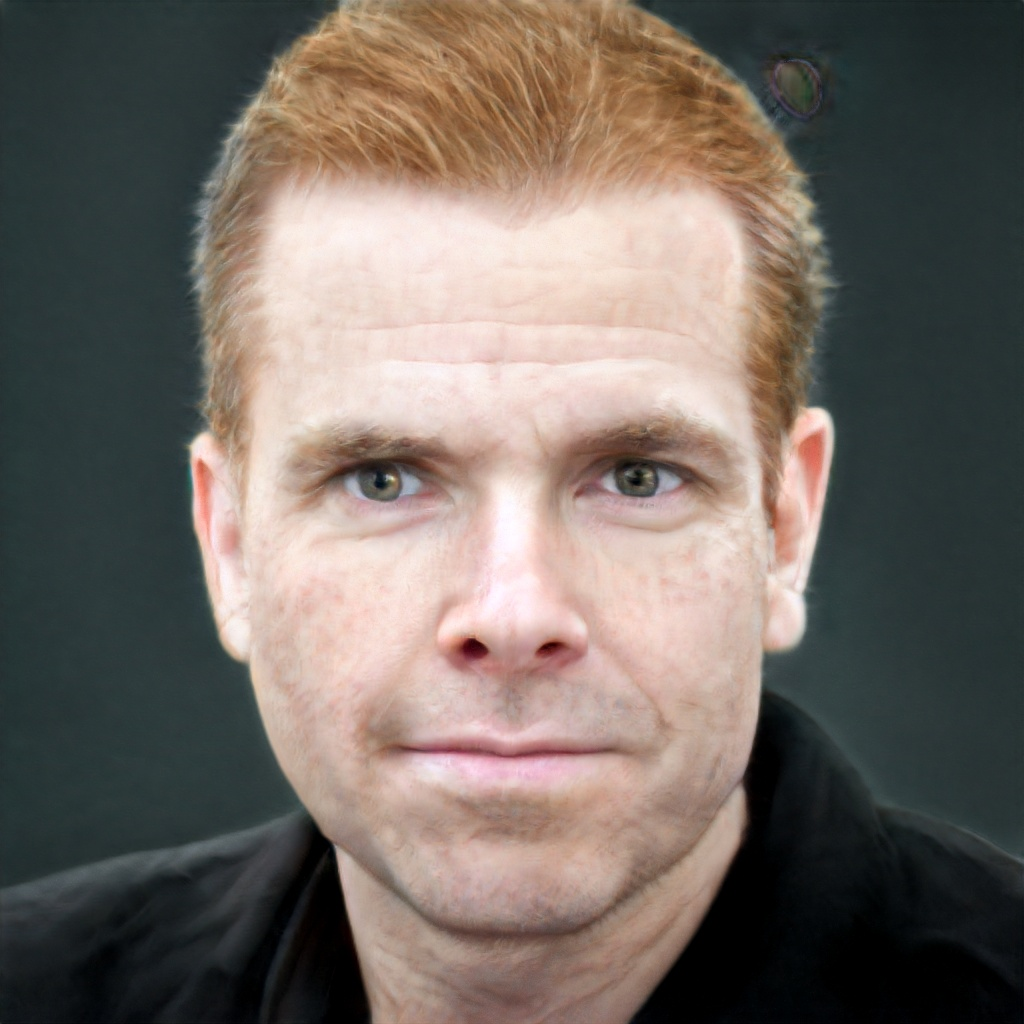
\includegraphics[width=\textwidth]{fig/stylegan/faceedit/inger-gender}
    \end{subfigure}
    \begin{subfigure}[b]{0.24\textwidth}
        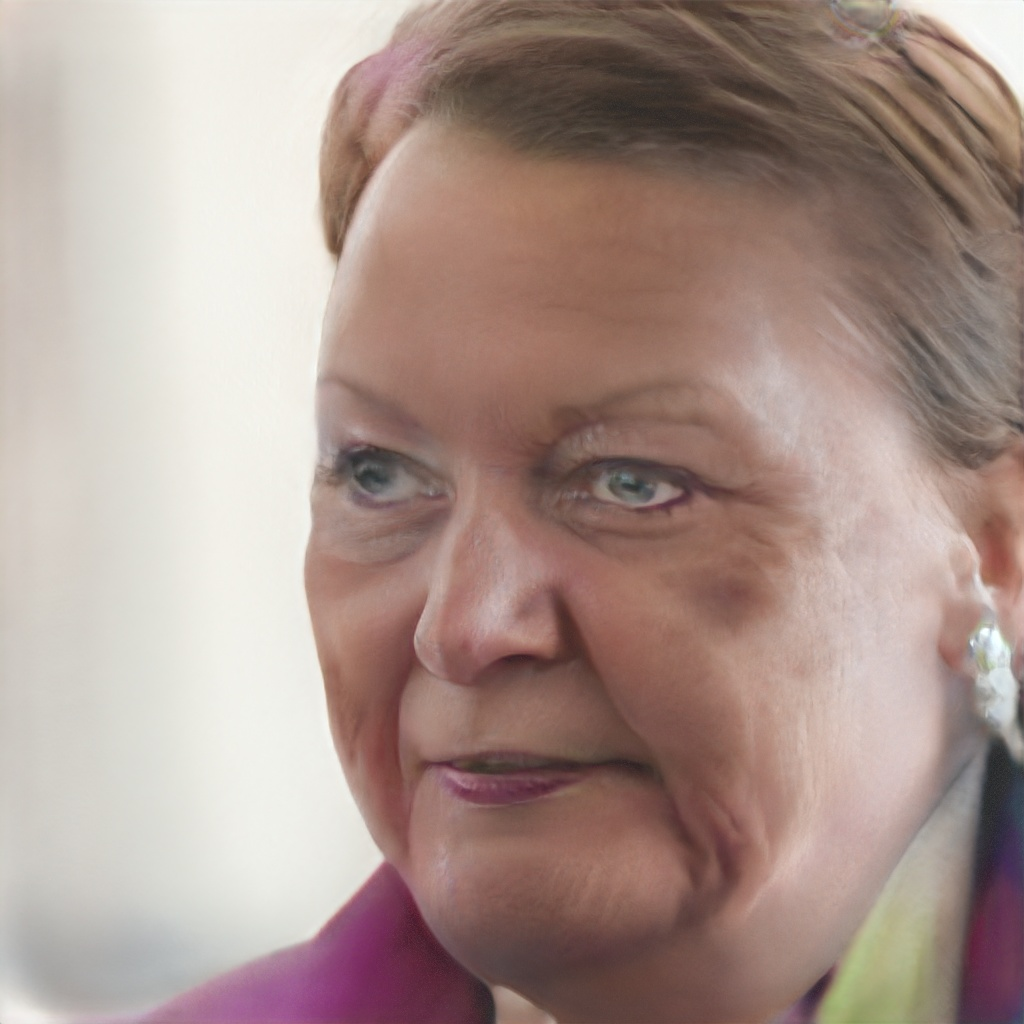
\includegraphics[width=\textwidth]{fig/stylegan/faceedit/lars-gender}
    \end{subfigure}
    \begin{subfigure}[b]{0.24\textwidth}
        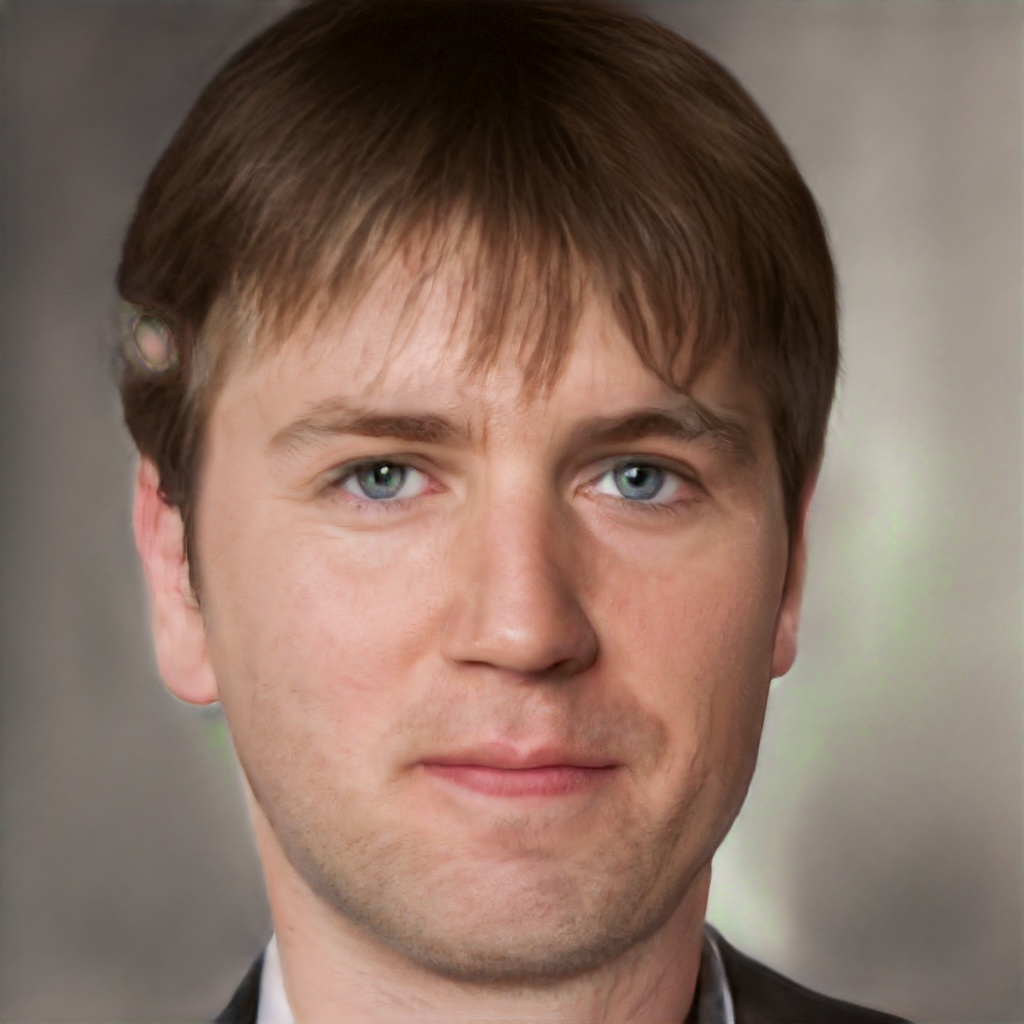
\includegraphics[width=\textwidth]{fig/stylegan/faceedit/mette-gender}
    \end{subfigure}
    \begin{subfigure}[b]{0.24\textwidth}
        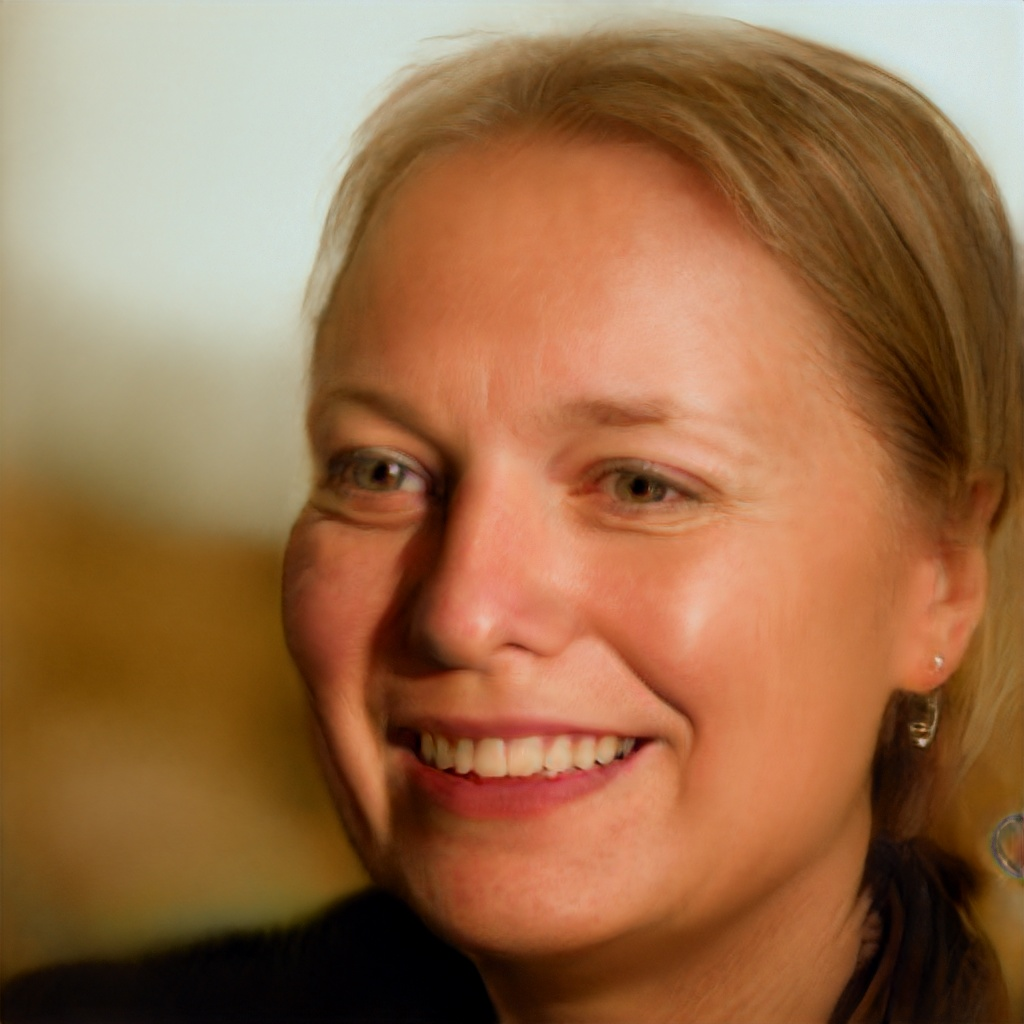
\includegraphics[width=\textwidth]{fig/stylegan/faceedit/uffe-gender}
    \end{subfigure}
    \caption{Semantic face editing.}
    \label{faceedit}
\end{figure}
